% Intuition and PCA
\begin{frame}{Intuition}
	\begin{minipage}{0.47\textwidth}
    		\begin{itemize}
        		\item Hypothetical test contains items related to openness and talkativeness.
			\item Notice the high correlation between variables.
    		\end{itemize}
	\end{minipage}
	\begin{minipage}{0.5\textwidth}
    		\begin{center}
        		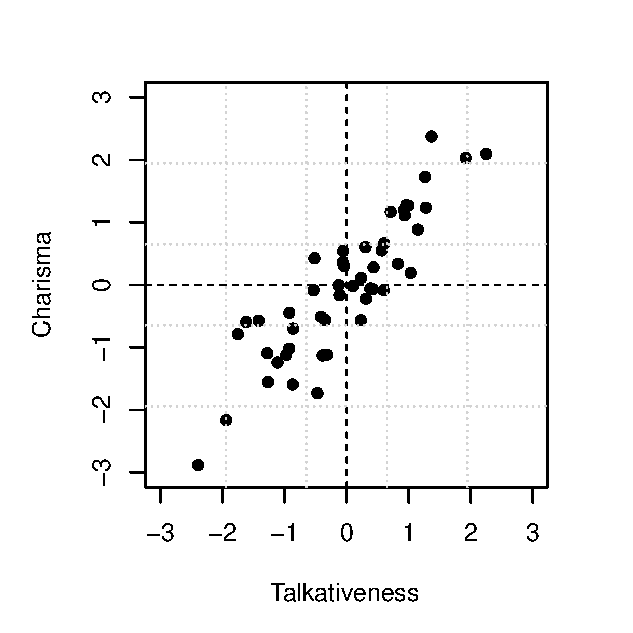
\includegraphics[scale=.6, left]{figures/pca1.eps}
    		\end{center}
	\end{minipage}
\end{frame}

\begin{frame}{Intuition}
	\begin{minipage}{0.47\textwidth}
    		\begin{itemize}
        		\item Score is measured in units of openness and talkativeness (called basis 
				  vectors)
    		\end{itemize}
	\end{minipage}
	\begin{minipage}{0.5\textwidth}
    		\begin{center}
        		\includegraphics<1>[scale=.6, left]{figures/pca2.eps}
			\includegraphics<2>[scale=.6, left]{figures/pca3.eps}
    		\end{center}
	\end{minipage}
\end{frame}

\begin{frame}{Intuition}
	\begin{minipage}{0.47\textwidth}
    		\begin{itemize}
        		\item Since variables are highly correlated, could create new axes along the 
					 dimension of maximum variance.
			\item Creates new variables which are \emph{composites} of the old ones.
    		\end{itemize}
	\end{minipage}
	\begin{minipage}{0.5\textwidth}
    		\begin{center}
        		\includegraphics<1>[scale=.6, left]{figures/pca1.eps}
			\includegraphics<2>[scale=.6, left]{figures/pca4.eps}
			\includegraphics<3>[scale=.6, left]{figures/pca5.eps}
    		\end{center}
	\end{minipage}
\end{frame}

\begin{frame}{Intuition}
	\begin{minipage}{0.47\textwidth}
    		\begin{itemize}
        		\item Replotting with the new axes reveals that most of the variability in the data 
				  lies along \emph{one-dimension}.
    		\end{itemize}
	\end{minipage}
	\begin{minipage}{0.5\textwidth}
    		\begin{center}
        		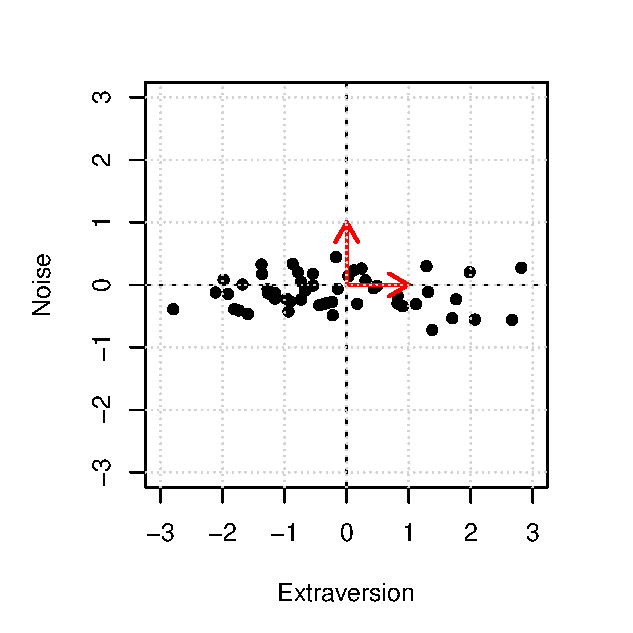
\includegraphics[scale=.6, left]{figures/pca6.eps}
    		\end{center}
	\end{minipage}
\end{frame}